\documentclass[11pt,titlepage]{article}

%Laenderspezifische Einstellungen bzgl. Rechtschreibung, Sonderzeichen und Kodierung
\usepackage[utf8]{inputenc}
\usepackage[naustrian]{babel}
\usepackage[T1]{fontenc}
\usepackage{titlesec}
\usepackage{graphicx}
%\usepackage{subcaption}

\usepackage{listings}
\usepackage{color}
\usepackage{courier}
\definecolor{light-gray}{gray}{0.85}
\definecolor{dark-green}{rgb}{0.05,0.65,0.3}
\lstset{
language=C++,
numbers=left,
breaklines=true,
backgroundcolor=\color{light-gray},
tabsize=2,
basicstyle=\footnotesize\ttfamily,
frame=single,
inputencoding=utf8,
extendedchars=true,
showstringspaces=false,
commentstyle=\color{dark-green}\ttfamily,
literate =
	{ä}{{\"a}}1
	{ö}{{\"o}}1
	{ü}{{\"u}}1
	{Ä}{{\"A}}1
	{Ö}{{\"O}}1
	{Ü}{{\"U}}1
	{ß}{{\ss}}1
	{ₙ}{{$_n$}}1
}

\def\ContinueLineNumber{\lstset{firstnumber=last}}
\def\StartLineAt#1{\lstset{firstnumber=#1}}

\usepackage[
	a4paper,
	top = 2cm,
	bottom = 2 cm,
	left = 2cm,
	right = 2cm,
	headheight = 15pt,
	includeheadfoot
	]{geometry}
\usepackage{fancyhdr}
\usepackage{amssymb}
\usepackage{amsmath}
\usepackage[english]{varioref}
\usepackage{hyperref}

\usepackage{float}
\usepackage{amsthm}

\fancypagestyle{fancy}{
	\fancyhead[R]{Seite \thepage}
	\fancyhead[L]{\leftmark}
	\renewcommand{\headrulewidth}{1.25pt}

	\fancyfoot[L]{\tiny{\textit{Mathematische Modelle in der Technik} - Schaltkreismodellierung}}
	\fancyfoot[R]{\tiny{ Felix Dreßler (k12105003)}}
	\cfoot{}
	\renewcommand{\footrulewidth}{1.25pt}
}

\setlength{\headsep}{10mm}
\setlength{\footskip}{10mm}

\setlength{\parindent}{0mm}
\setlength{\parskip}{1.1ex plus0.25ex minus0.25ex}
\setlength{\tabcolsep}{0.2cm} % for the horizontal padding

\pagestyle{fancy}

\title{Seminar zu \textit{Mathematische Modelle in der Technik} - Schaltkreismodellierung}
\author{Felix Dreßler (k12105003)\\ email \href{mailto:FelixDressler01@gmail.com}{FelixDressler01@gmail.com}}
\date{\today} %Erstellungsdatum

\renewcommand{\labelenumi}{\roman{enumi})}

\begin{document}
\maketitle

	\tiny{Die Informationen in diesem Dokument stammen hauptsächlich aus dem Buch C. Eck, H. Garcke, P. Knabner, Mathematische Modellierung, Springer (2017) sowie der Vorlesung (Johannes Kepler Universität, Linz) Special Topics Numerical Analysis, Herbert Egger.}
	
	\normalsize

	\section{Elektrische Netzwerke, Gleichstromkreis}
		Elektrische Netzwerke findet man heutzutage in fast allen technischen Anwendungen. Sie bestehen üblicherweise aus einer durch Leiter verbundenen Kombination von Widerständen, Spulen, Kondensatoren, Strom- und Spannungsquellen sowie weitere Bauteile wie Dioden oder Transistoren auf welche wir hier jedoch nicht genauer eingehen. Ein Beispiel für ein elektrisches Netzwerk ist folgendes Netzwerk aus Widerständen und Spannungsquellen.
		\begin{figure}[ht]
			\centering
			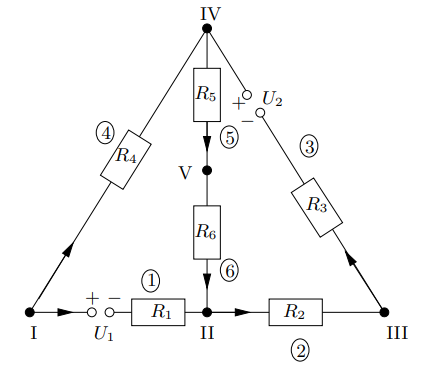
\includegraphics[scale=0.7]{Photos/ElektrNEt.png}
			\caption{Elektrisches Netzwerk}
		\end{figure}
	
		Wichtige Größen in der Elektrotechnik und Elektronik sind unter anderem
		\begin{itemize}
			\item Strom [I] = A ... Ampere
			\item Spannung [U] = V ... Volt
			\item Widerstand [R] = $\frac{V}{A}$ = $\Omega$ ... Ohm
		\end{itemize}
		Ein Ampere entspricht dem Fluss von einem Coulomb pro Sekunde, wobei ein Coulomb $6,24150965 * 10^{18}$ Elementarladungen entspricht. Die Spannung ist die Ursache des Stromflusses und gibt die \glqq Stärke\grqq{} einer Spannungsquelle an. Der Widerstand ist ein Maß, für die nötige Spannung um eine bestimmte elektrische Stromstärke durch einen Leiter fließen zu lassen.
		In der Wechselstromtechnik werden wir später noch Induktivität und Kapazität verwenden.

		In diesem Kapitel beschäftigen wir uns vorerst nur mit Gleichstromnetzwerken. Das heißt dass alle vorkommenden Spannungen zeitlich konstant sind.
					
	\subsection{Mathematische Modellierung}
		Zur Modellierung solch eines Netzwerks definiert man eine beliebige Nummerierung der Knoten und Kanten. Ebenso legt man eine \textit{positive} Stromrichtung in jeder Kante fest. Diese Stromrichtung sagt nichts über die tatsächliche Flussrichtung aus, sie dient lediglich zur mathematischen Darstellung. Die Modellierung eines Netzwerks über solche Knoten (oder Englisch Nodes) bezeichnet man auch als Modified-Nodal-Analysis. Modified deshalb, weil man bei der klassischen Modal-Analysis nur die Spannungen, nicht aber die Ströme berechnen würde.
		
		Mit Hilfe dieser Knoten und Kanten lassen sich nun drei wichtige physikalische Gesetze formulieren:
		
		\begin{itemize}
			\item Ohmsches Gesetz
			\subitem Dieses Gesetz gibt uns einen Zusammenhang zwischen der an einem Widerstand abfallenden Spannung und dem durch den Widerstand fließenden Strom.
			\subitem $U = R*I$
			\item Kirchhoffsches Stromgesetz
			\subitem Dieses Gesetz Beschreibt die Erhaltung der elektrischen Ladung innerhalb eines "Knotens". In einem Knoten ist die Summe aller eingehenden Ströme gleich der Summe aller ausgehenden Ströme.
			\item Kirchhoffsches Spannungsgesetz
			\subitem Dieses Gesetz gibt Aufschluss über die auftretenden Spannungen in einer \textit{Schleife} bzw. \textit{Masche}. Eine Masche ist ein geschlossener Umlauf zwischen Knoten eines elektrischen Netzwerks, welcher keine Kanten im Inneren enthält. Das Kirchhoffsche Spannungsgesetz sagt nun, dass die Summe aller in einer Masche auftretenden Spannungen Null ist.
		\end{itemize}	
		
		Weiters werden Variablen für alle unbekannten Größen eingeführt. Diese Variablen unterteilen wir in:
		
		\begin{itemize}
			\item Knotenvariablen
			\subitem In einem Vektor $x = (x_1, ..., x_m)$ werden die Potentiale an den Knoten zusammengefasst.
			\item Kantenvariablen
			\subitem In einem Vektor $y = (y_1, ..., y_n)$ werden die Ströme der Kanten zusammengefasst.
		\end{itemize}
		
		Die Spannungen $e = (e_1, ..., e_n)$ berechnen sich aus den Potentialen über $e_i = x_{u(i)} - x_{o(i)}$ wobei $u(i)$ den \glqq unteren\grqq{} und $o(i)$ den \glqq oberen\grqq{} Index einer Kante bezüglich der Stromrichtung angibt.
				
		Die Beziehung zwischen Potentialen und Spannungen lässt sich schreiben als 
		\begin{displaymath}
			e = -Bx
		\end{displaymath}
		Wobei sich B Komponentenweise definieren lässt als
		\begin{displaymath}
			b_{ij} = 
			\begin{cases}
				1 &  j = o(i) \\
				-1 &  j = u(i) \\
				0 & sonst				
			\end{cases}
		\end{displaymath}
		
		B nennt man Inzidenzmatrix.
		
		Der Zusammenhang zwischen Strom- und Spannungsvektor ist durch das Ohmsche Gesetz gegeben. Dabei sind natürlich Spannungsquellen zu berücksichtigen. Die folgende Abbildung zeigt ein Leiterstück mit Widerstand und Spannungsquelle.
		
		\begin{figure}[H]
			\centering
			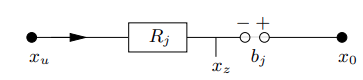
\includegraphics[scale=0.7]{Photos/Example1.png}
			\caption{Leiterstück mit Widerstand und Spannungsquelle}
		\end{figure}
		
		 Für die Potentiale $x_u$, $x_z$, $x_o$ gilt mit der Spannung $b_j$ der Spannungsquelle:
		\begin{displaymath}
			x_z = x_u - R_j y_j \qquad x_o = x_z + b_j
		\end{displaymath}
		Und damit
		\begin{displaymath}
			e_j = x_u - x_o = R_j y_j - b_j
		\end{displaymath}
	
		$R_j y_j$ bezeichnet hier also den Spannungsabfall am Widerstand und $b_j$ die von der Spannungsquelle zusätzlich erzeugte Potentialdifferenz. In Vektroschreibweise erhält man also
		
		\begin{displaymath}
			y = C(e+b)
		\end{displaymath}
		
		Wobei $C \in \mathbb{R}^{n \times n}$ eine Diagonalmatrix ist, deren Einträge die Leitwerte $R_j^{-1}$ enthalten. Das Kirchhoffsche Gesetz lässt sich in Vektorschreibweise schreiben als
		
		\begin{displaymath}
			Ay = 0
		\end{displaymath}
		wobei $A$ definiert ist als
		\begin{displaymath}
			a_{ij} = 
			\begin{cases}
				1 &  i = o(j) \\
				-1 &  i = u(j) \\
				0 & sonst				
			\end{cases}
		\end{displaymath}
		Im Vergleich mit der Inzidezmatrix $B$ erkennt man, dass $A = B^T$.
		Das Kirchhoffsche Spannungsgesetz wurde durch den Potentialvektor $x$ bereits in das System eingebaut.
		
		Zusammenfassend ist die Modellierung eines elektrischen Netzwerks mit $m$ Knoten und $n$ Leitungen bestimmt durch:
		\begin{itemize}
			\item einen Potentialvektor $x \in \mathbb{R}^m$,
			\item einem Spannungsvektor $e \in \mathbb{R}^n$ der aus der Inzidenzmatrix $B \in \mathbb{R}^{n \times m}$ über $e = -Bx$ berechnet wird,
			\item einem Stromvektor $y \in \mathbb{R}^n$ der durch $y = C(e+b)$ mit einer Leitwertmatrix $C \in \mathbb{R}^{n \times n}$ und dem Spannungquellenvektor $b \in \mathbb{R}^n$ berechnet wird
			\item dem Kirchhoffschen Spannungsgesetz $B^T y = 0$.
		\end{itemize}
	
		Die Inzidenzmatrix hält dabei die Geometrie des Netzwerkes, die Leitwertmatrix die Materialeigenschaften und der Vektor $b$ die \grqq außeren Triebkräfte\glqq{} fest.
		
		Zur Berechnung der Ströme, Spannungen und Potentiale im Netzwerk wählt man eine zu bestimmende Variable, zum Beispiel x, und leitet duch Kombination obiger Beziehungen eine Gleichung für x her. 
		Durch einsetzen erhält man
		\begin{displaymath}
			B^T C (b-Bx)=0
		\end{displaymath}
		und durch anschließenden ausmultiplizieren und umformen
		\begin{displaymath}
			B^T C Bx = B^T C b
		\end{displaymath}
	
		Die Matrix $M = B^T C B$ ist symmetrisch, falls C symmetrisch ist. Aus
		\begin{displaymath}
			\langle x,Mx \rangle = \langle Bx, CBx \rangle
		\end{displaymath}
		Mit dem euklidischen Skalarprodukt sieht man, dass
		\begin{itemize}
			\item $C$ positiv semidefinit $\Rightarrow$ $M$ positiv Semidefinit
			\item $C$ positiv definit und $ker(B)= \{ 0 \}$ $\Rightarrow$ $M$ positiv definit
		\end{itemize}
	
		Für die meisten Netzwerke ist C auch wirklich positiv definit. Die Inzidenzmatrix hat jedoch einen nichttrivialen Kern. Man sieht leicht, dass $(1,...,1)^T \in \mathbb{R}^m$ im Kern von $B$ liegt. (Das gilt für jede Inzidenzmatrix) Das lineare Gleichungssystem hat deshalb keine eindeutige Lösung. Physikalisch ist das leicht einzusehen: Die Potentiale sind nur bis auf eine Konstante bzw. einen gemeinsamen Nullpunkt eindeutig.
		
		Zur Lösbarkeit gilt jedoch folgendes Resultat aus der Algebra:
		
		\newtheorem{Satz}{Satz}
		\begin{Satz}
			Sei $C \in \mathbb{R}^{n \times n}$ symmetrisch und positiv definit und $B \in \mathbb{R}^{n \times m}$ dann gilt für $M = B^TCB$:
			\begin{enumerate}
				\item $ker(M) = ker(B)$
				\item Das Gleichungssystem $Mx = B^Tb$ hat für jedes $b \in \mathbb{R}^n$ eine Lösung.
			\end{enumerate}
		\end{Satz}
		\begin{proof}
			i) Aus der Definition von $M$ sieht man sofort, dass $ker(B) \subseteq ker(M)$.
			Umgekehrt gilt für $x \in ker(M)$
			\begin{displaymath}
				0 = \langle x, B^TCBx \rangle = \langle Bx, CBx \rangle
			\end{displaymath}
			Weil aber C positiv definit ist, muss $Bx = 0$ gelten und somit $x \in ker(B)$.
			
			ii) Die Gleichung ist Lösbar, falls $B^Tb \perp ker(M^T)$ gilt. Weil $C$ symmetrisch ist, gilt auch, dass $M$ symmetrisch ist. Für $x \in ker(M^T) = ker(M) = ker(B)$ gilt
			\begin{displaymath}
				\langle B^Tb, x \rangle = \langle b, Bx \rangle = 0
			\end{displaymath}
			womit die Aussage bewiesen ist.
		\end{proof}
		
		\newtheorem{Bemerkung}{Bemerkung}
		\begin{Bemerkung}
			Da $C$ vollen Rang hat, reicht es in obigem Satz die Lösbarkeit des Gleichungssystems $Mx = B^Tb$ anstatt $Mx = B^TCb$ zu zeigen.
		\end{Bemerkung}
		
		\newtheorem{Definition}{Definition}
		\begin{Definition}
			Ein Netzwerk heißt zusammenhängend, wenn je zwei Knoten durch einen Weg aus Kanten verbunden sind.
		\end{Definition}
	
		Äquivalente Kriterien dazu liefert folgender Satz welchen wir hier nicht beweisen werden.

		\begin{Satz}
			Für ein Netzwerk mit Inzidenzmatrix $B$ sind folgende Aussagen äquivalent:
			\begin{enumerate}
				\item Das Netzwerk ist zusammenhängend
				\item B kann nicht durch Umsortieren von Zeilen und Spalten in die Form
					\begin{displaymath}
						B = 
						\left( 
						\begin{matrix}
							B_1 & 0 \\
							0 & B_2
						\end{matrix}
						\right)
					\end{displaymath}
					gebracht werden.
				\item $ker(B) = span{(1,...,1)^T}$
			\end{enumerate}
		\end{Satz}
	\newpage
	\section{Wechselstromkreise}
	
		Im Wechselstromkreis hat man zeitlich oszillierenden Strom mit vorgegebener Frequenz $\omega$, also
		\begin{displaymath}
			I(t) = I_0 cos(\omega t)
		\end{displaymath}
		
		Das Ohmsche Gesetz schreibt sich dann als
		\begin{displaymath}
			U(t) = R I_0 cos(\omega t) = U_0 cos(\omega t) \qquad U_0 = R I_0
		\end{displaymath}
		
		Wir erkennen also, dass ein Wechselstromkreis der nur Widerstände und keine weiteren Bauteile enthält anhand der Amplituden genauso simuliert werden kann wie ein Gleichstromkreis. Neue Effekte kommen jedoch durch weitere elektrische Bauteile ins Spiel.
		
		\begin{itemize}
			\item Kondensatoren
			\subitem Ein Kondensator kann elektrische Ladungen speichern. Die Menge der gespeicherten Ladung ist proportional zur angelegten Spannung. Bei Spannungsänderung nimmt ein Kondensator daher Ströme auf bzw. gibt diese ab. Dies wird durch
			\begin{displaymath}
				I(t) = C \dot{U} (t)
			\end{displaymath}
			beschrieben, wobei $C$ die Kapazität des Kondensators ist. In einem Wechselstromkreis mit obiger Stromform gilt also
			\begin{displaymath}
				U(t) = \frac{I_0}{C \omega}sin(\omega t) = \frac{I_0}{C \omega} cos(\omega t - \frac{\pi}{2})
			\end{displaymath}
			Der Kondensator verursacht also eine Phasenverschiebung um $-\frac{\pi}{2}$ zwischen Strom und Spannung.
			\item Spulen
			\subitem Eine Stromdurchflossene Spule erzeugt ein Magnetfeld, dessen Stärke proportional zur Stromstärke ist. In diesem Magnetfeld ist Energie gespeichert, diese Muss beim Aufbau des Magnetfeldes aus dem Strom der Spule entnommen werden. Dadurch entsteht ein Spannungsabfall an der Spule, der proportional zur Änderung der Stromstärke ist
			\begin{displaymath}
				U(t) = L \dot{I}(t)
			\end{displaymath}
			$L$ beschreibt die Induktivität der Spule. Im Wechselstromkreis gilt also
			\begin{displaymath}
				U(t) = -L I_0 \omega sin(\omega t) = L \omega I_0 cos(\omega t + \frac{\pi}{2})
			\end{displaymath}
			Es tritt also eine Phasenverschiebung um $+\frac{\pi}{2}$ auf.
		\end{itemize}
	
		Diese Phasenverschiebungen machen die Berechnungen komplizierter. Zur Darstellung von Strom und Spannung ist es nützlich komplexe Zahlen zu verwenden. Man nutzt dazu die Eulersche Formel.
		\begin{displaymath}
			e^{i \phi} = cos(\phi ) +i sin(\phi)
		\end{displaymath}
		Damit gilt
		\begin{displaymath}
			cos(\omega t) = Re(e^{i \omega t}) \qquad sin(\omega t) = Re(-i e^{i \omega t})
		\end{displaymath}
		Für den Strom gilt damit
		\begin{displaymath}
			I(t) = I_0 Re(e^{i \omega t})
		\end{displaymath}
		und für die Spannungsabfälle
		\begin{itemize}
			\item am ohmschen Widerstand $U(t) = Re(R I_0 e^{i \omega t})$
			\item am Kondensator $U(t) = Re(- \frac{i}{\omega C} I_0 e^{i \omega t})$
			\item an der Spule $U(t) = Re(i \omega L I_0 e^{i \omega t})$
		\end{itemize}
		Man kann dies durch komplexe Impedanzen $R$, $-\frac{i}{\omega C}$, $i \omega L$ darstellen, diese übernehmen die Rolle der reellen Widerstände. Sind diese Bauteile auf einem Leiterstück \grqq in Serie \glqq{} eingebaut kann man wie bei reellen Widerständen die komplexen Impedanzen addieren.
	
	\newpage
	\section{Ein Beispiel (Zeitharmonischer Ansatz)}
		
		\begin{figure}[H]
			\centering
			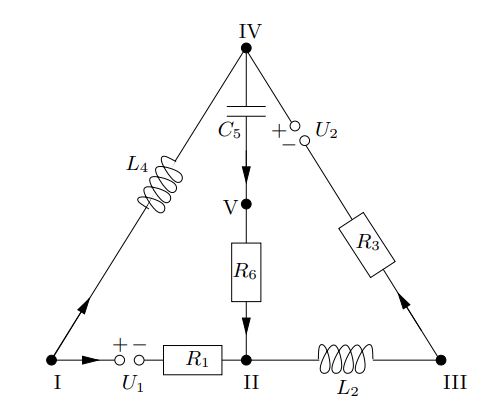
\includegraphics[scale=0.7]{Photos/Beispiel}
			\caption{Elektrisches Netzwerk mit Kondensatoren und Spulen}
		\end{figure}
				
		Wir betrachten ein Beispiel mit $m=5$ Knoten und $n=6$ Kanten. In der Skizze sind bereits Nummerierungen und positive Stromrichtungen vorgegeben. Die angelegten Spannungen sind gegeben durch
		\begin{displaymath}
			U_1(t) = U_{01} cos(\omega t) \qquad
			U_2(t) = U_{02} cos(\omega t)
		\end{displaymath}
		Wichtig ist hier, dass beide Spannungen die gleiche Frequenz haben, sonst liegt kein Wechselstromnetz mit bekannter Frequenz vor. Phasenverschiebungen können jedoch mit einigen Überlegungen ins Modell eingebaut werden.
		Weiters benötigen wir zur Modellierung noch
		\begin{description}
			\item einen Potentialvektor $x \in \mathbb{C}^{m}$
			\item einen Stromvektor $y \in \mathbb{C}^{n}$
			\item und einen Spannungsvektor $e \in \mathbb{C}^n$.
		\end{description}
		Es gilt
		\begin{displaymath}
			e = -Bx \qquad
			y = C(e+b)
		\end{displaymath}
		
		Die Inzidenzmatrix $B$, die Impedanzmatrix $C$ und der Spannungsvektor $b$ haben folgende Form:
		
		\begin{displaymath}
			C^{-1}=
			\begin{pmatrix}
				R_1 & 0 & 0 & 0 & 0 & 0 \\
				0 & i \omega L_2 & 0 & 0 & 0 & 0 \\
				0 & 0 & R_3 & 0 & 0 & 0 \\
				0 & 0 & 0 & i \omega L_4 & 0 & 0 \\
				0 & 0 & 0 & 0 & \frac{1}{i \omega C_5} & 0 \\
				0 & 0 & 0 & 0 & 0 & R_6
			\end{pmatrix}
			\qquad
			B=
			\begin{pmatrix}
				-1 & 1 & 0 & 0 & 0 \\
				0 & -1 & 1 & 0 & 0 \\
				0 & 0 & -1 & 1 & 0 \\
				-1 & 0 & 0 & 1 & 0 \\
				0 & 0 & 0 & -1 & 1 \\
				0 & 1 & 0 & 0 & -1
			\end{pmatrix}
			\qquad
			b=
			\begin{pmatrix}
				-U_{01} \\
				0 \\
				U_{02}\\
				0 \\
				0 \\
				0
			\end{pmatrix}	
		\end{displaymath}
		Man erhält wie beim GLeichstrom dieselben Gleichungssysteme, mit dem einzigen Unterschied, dass die Koeffizienten in $C$ und $b$ nun im Allgemeinen komplexe Zahlen sind.
		
		Für explizite Werte seinen nun $R_1 = R_3 = R_6 = 1 \Omega$, $L_2 = L_4 = 0,01 H$, $C_5 = 0,02 F$, $\omega = 50 Hz$ sowie $U_{01} = 10 V$, $U_{02} = 5 V$.
		Ohne Einheiten folgt
		
		\begin{displaymath}
			C = diag(1, -2i, 1, -2i, i, 1) \qquad b = (-10, 0, 5, 0, 0, 0)^T
		\end{displaymath}
		
		Damit hat das Gleichungssystem $B^T C B x = B^T C b$ die Form
		
		\begin{displaymath}
			\begin{pmatrix}
				1-2i & -1 & 0 & 2i & 0 \\
				-1 & 2-2i & 2i & 0 & -1 \\
				0 & 2i & 1-2i & -1 & 0 \\
				2i & 0 & -1 & 1-i & -i \\
				0 & -1 & 0 & -i & 1+i \\
			\end{pmatrix}
			x=
			\begin{pmatrix}
				10 \\
				-10 \\
				-5\\
				5 \\
				0
			\end{pmatrix}
		\end{displaymath}
		
		mit der allgemeinen Lösung
		
		\begin{displaymath}
			x=
			\begin{pmatrix}
				2i \\
				2i-6 \\
				2i-5 \\
				0 \\
				4i-2
			\end{pmatrix}
			+ z
			\begin{pmatrix}
				1 \\
				1 \\
				1 \\
				1 \\
				1
			\end{pmatrix}
		\end{displaymath}
		mit $z \in \mathbb{C}$
		
		Daraus lassen sich Spannungen und Ströme berechnen:
		
		\begin{displaymath}
			e = -Bx = 
			\begin{pmatrix}
				6 \\
				-1 \\
				2i-5 \\
				2i \\
				2-4i \\
				4+2i
			\end{pmatrix}
			\qquad
			y = C(e+b) = 
			\begin{pmatrix}
				-4 \\
				2i \\
				2i \\
				4 \\
				4+2i \\
				4+2i
			\end{pmatrix}
		\end{displaymath}
		Den zeitlichen Verlauf einer komplexen Zahl $c \in \mathbb{C}$ erhält man durch $c(t) = Re(ce^{i \omega t})$. Beispielsweise hat der Strom in Leiter 5 die Form
		\begin{displaymath}
			y_5 (t) = Re((4+2i)e^{i \omega t}) = 4 cos(\omega t) - 2 sin(\omega t)
		\end{displaymath}
	
		Liegen zwischen den Spannungen Phasenverschiebungen vor, so erhält man im Vektor $b$ komplexe Einträge. Ist beispielsweise $U_2 (t) = U_{02} sin(\omega t)$ dann gilt $U_2 (t) = Re(-iU_{02}e^{i \omega t})$ und somit
		\begin{displaymath}
			b=
			\begin{pmatrix}
				-U_{01} \\
				0 \\
				-iU_{02}\\
				0 \\
				0 \\
				0
			\end{pmatrix}
		\end{displaymath}
	\newpage
	\section{Differential Algebraische Gleichungen}
		\subsection{Was sind Differential Algebraische Gleichungen (DAE - Differential Algebraic Equations)}
		Die Modellierung dynamischer Systeme bzw. Prozesse führt typischerweise auf mathematische Modelle, die Differential- und algebraische Gleichungen beinhalten.
		
		In abstrakter Form lassen sich diese schreiben als 
		$\qquad F(t, y(t), \dot{y}(t)) = 0$ \newline
		mit $F:\mathbb{R} \times \mathbb{R}^n \times \mathbb{R}^n \to \mathbb{R}^n$ hinreichend glatt und $y:\mathbb{R} \to \mathbb{R}^n$.
		
		Um eine Lösung eindeutig festzulegen müssen dann ebenso geeignete Anfangswerte gegeben werden.
		
		Diese Form der Gleichung ist aber of zu allgemein um eine einheitliche Behandlung zu ermöglichen. Deshalb versucht man stattdessen Probleme mit spezieller Struktur zu betrachten. Es gibt mehrere Arten von Differentialalgebraischen Gleichungen. Eine davon ist ein System mit konstanten Koeffizienten. Diese haben die Form
		
		\begin{displaymath}
			E \dot{u}(t) = A u(t) + f(t)
		\end{displaymath}
		
		mit $E, A \in \mathbb{R}^{n \times n}$ und $f:\mathbb{R} \to \mathbb{R}^n$ hinreichend glatt.
		
		\subsection{Beispiel: Laden eines Kondensators}
		
		Ein Beispiel für ein elektrisches Netzwerk welches als Modell eine lineare DAE besitzt ist das laden eines Kondensators.
		
		\begin{figure}[H]
			\centering
			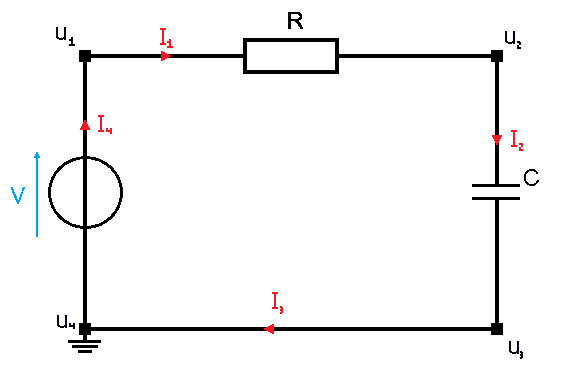
\includegraphics[scale=0.7]{Photos/Kondensator}
			\caption{Laden eines Kondensators}
		\end{figure}
		
		Vorab lassen sich direkt einige Beobachtungen machen.
		\begin{enumerate}
			\item Weil alle Knoten nur eine eingehende und eine ausgehende Kante besitzen liefert uns die Kirchhoffsche Knotenregel, dass
				\begin{displaymath}
					I_1 = I_2 = I_3 = I_4
				\end{displaymath}
			\item Da die Kante 3 keine Bauteile enthält (Kurzschluss) gilt 
				\begin{displaymath}
					u_3 = u_4
				\end{displaymath}
			\item Der Spannungsabfall am Widerstand ist gegeben durch 
				\begin{displaymath}
					u_2 - u_1 = R I_1
				\end{displaymath}
			\item Für den Kondensator gilt
				\begin{displaymath}
					I_2 = C(\dot{u}_3 - \dot{u}_2)
				\end{displaymath}
			\item Für die Spannungsquelle gilt
				\begin{displaymath}
					u_1 - u_4 = V(t)
				\end{displaymath}
			\item Aufgrund der Erdung gilt
				\begin{displaymath}
					u_4 = 0
				\end{displaymath}
		\end{enumerate}
		Daraus folgt ein System für $u_1, u_2, I_3$
		\begin{displaymath}
			\begin{pmatrix}
				0 & 0 & 0 \\
				0 & C & 0 \\
				0 & 0 & 0
			\end{pmatrix}
			\begin{pmatrix}
				\dot{u}_1 \\
				\dot{u}_2 \\
				\dot{I}_3
			\end{pmatrix}
		 	=
		 	\begin{pmatrix}
		 		1 & -1 & R \\
		 		0 & 0 & -1 \\
		 		-1 & 0 & 0
		 	\end{pmatrix}
	 		\begin{pmatrix}
	 			u_1 \\
	 			u_2 \\
	 			I_3 
	 		\end{pmatrix}
 			+
 			\begin{pmatrix}
 				0 \\
 				0 \\
 				V(t)
 			\end{pmatrix}
		\end{displaymath}
		welches die Form $Ey' = Ay + f(t)$ hat und somit eine lineare DAE mit konstanten Koeffizienten ist.
\end{document}